\documentclass[letterpaper,11pt]{article}
\oddsidemargin -1.0cm \textwidth 17.5cm

\usepackage[utf8]{inputenc}
\usepackage[activeacute,spanish, es-lcroman]{babel}
\decimalpoint
\usepackage{amsfonts,setspace}
\usepackage{amsmath}
\usepackage{amssymb, amsmath, amsthm}
\usepackage{comment}
\usepackage{float}
\usepackage{amssymb}
\usepackage{dsfont}
\usepackage{anysize}
\usepackage{multicol}
\usepackage{enumerate}
\usepackage{graphicx}
\usepackage[left=1.5cm,top=2cm,right=1.5cm, bottom=1.7cm]{geometry}
\setlength\headheight{1.5em} 
\usepackage{fancyhdr}
\usepackage{multicol}
\usepackage{hyperref}
\usepackage{wrapfig}
\usepackage{subcaption}
\usepackage{siunitx}
\usepackage{cancel}
\usepackage{mdwlist}
\usepackage{svg}
\pagestyle{fancy}
\fancyhf{}
\renewcommand{\labelenumi}{\normalsize\bfseries P\arabic{enumi}.}
\renewcommand{\labelenumii}{\normalsize\bfseries (\alph{enumii})}
\renewcommand{\labelenumiii}{\normalsize\bfseries \roman{enumiii})}


\begin{document}

\fancyhead[L]{\itshape{Facultad de Ciencias F\'isicas y Matem\'aticas}}
\fancyhead[R]{\itshape{Universidad de Chile}}
\rfoot[]{pág. \thepage}

\begin{minipage}{11.5cm}
    \begin{flushleft}
        \hspace*{-0.6cm}\textbf{FI1100 Introducción a la Física Moderna}\\
        \hspace*{-0.6cm}\textbf{Tutor:} Alejandro Cartes
    \end{flushleft}
\end{minipage}

\begin{picture}(2,3)
    \put(366, -10){
\includegraphics[scale=0.9]{Imágenes/logo/dfi-fcfm.pdf}}
\end{picture}

\begin{center}
	\LARGE\textbf{Tutoría C2}\\
	\Large{MAS y Ondas}
\end{center}

\vspace{-1cm}
\begin{enumerate}\setlength{\itemsep}{0.4cm}

\item[]


\rfoot[]{pág. \thepage}

\item Una partícula con carga eléctrica $-q$ se ubica entre dos partículas fijas con cargas $+q_1$ y $+q_2$ separadas a una distancia $R$. Considerando que la magnitud de la fuerza eléctrica entre dos cargas $q_1$ y $q_2$ separadas a una distancia $r$ es:
$$F_e = \frac{K q_1 q_2}{r^2}$$

\begin{enumerate}
    \item Determine la posición de equilibrio de la carga negativa

    \item Si la carga negativa se perturba una distancia vertical $\delta y$ pequeña desde su posición de equilibrio, demuestre que la partícula seguirá un movimiento armónico

    \item Determine la frecuencia de oscilación y la velocidad máxima de la partícula

    \item Si la carga se perturbara horizontalmente una distancia $\delta x$, ¿seguirá un movimiento armónico?
\end{enumerate}

\item Un péndulo simple de largo $L$ y masa $m$ cuelga del techo del interior de un camión que se desplaza en dirección horizontal con aceleración constante $a$. Calcule su período para pequeñas oscilaciones en torno a su posición de equilibrio

\item Considere una onda viajera descrita por:
\[ y(x,t) = 2\exp\left(\cos\left(-x-0.5t\right)\right)\]
    \begin{enumerate}
        \item Demuestre que $y(x,t)$ es solución a la ecuación de ondas.
        \item Determine sentido de propagación, velocidad, longitud de onda y periodo.
        \item Determine la velocidad transversal de la cuerda
    \end{enumerate}

\begin{minipage}{0.6\linewidth}
    \item Una cuerda  de  masa  $m$  y  largo  $L$  sostiene  un  bloque  de  masa  $M$,  como  se  indica  en la  figura. La distancia entre el extremo fijo y la polea es $l$. El bloque oscila libre de roce hasta un ángulo  máximo  $\theta$.
\end{minipage}
\hfill
\begin{minipage}{0.35\linewidth}
    \begin{figure}[H]
        \centering
        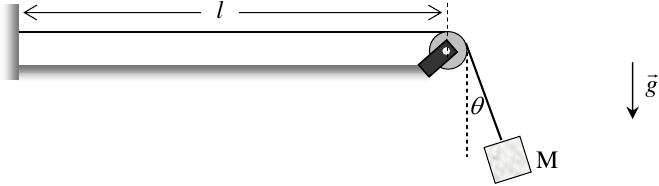
\includegraphics[width = 1\linewidth]{Imágenes/aux4/cuerda-pendulo.png}
    \end{figure}
\end{minipage}

Determine,  para  un  pulso  que  viaja  a  través  de  la  cuerda  horizontal,  el  tiempo  de  viaje  cuando  el  péndulo pasa  por  la  parte  más  baja  y  cuando  está  en  el  ángulo  máximo. Compare  los  resultados  e  indique en  cuál  condición  el  pulso  tarda  menos  tiempo.

\item Una cuerda de guitarra de longitud $L= \SI{0.7}{m}$ y densidad lineal de masa $\rho_L = \SI{7}{g/m}$ emite una nota de frecuencia $f=\SI{190}{Hz}$ en su primer modo de oscilación.
    \begin{enumerate}
        \item Determine la longitud de onda del modo fundamental de oscilación.
        \item Calcule la velocidad con que se propagan las ondas en la cuerda.
        \item Determine la tensión de la cuerda.
        \item Calcule la frecuencia de oscilación de los siguientes tres modos de oscilación de la cuerda.
        \item El mástil de la guitarra tiene varios trastes que permiten presionar la cuerda para disminuir la longitud efectiva de la misma. El primero está ubicado a una distancia de $\SI{0.04}{m}$ del extremo de la cuerda. ¿Qué frecuencia emite la cuerda en su modo fundamental al presionar sobre este traste?
        \item Se quiere afinar la cuerda para que entregue una nota sol ($f = \SI{196}{Hz}$) al oscilar en su modo fundamental. ¿Qué tensión se debe dar a la cuerda para lograr afinar la cuerda?
    \end{enumerate}

\end{enumerate}
\end{document}


% Para imágenes vectoriales -> el texto tiene que estar en LaTeX
% \begin{figure}[htbp]
%   \centering
%   \svgpath{../Imagenes/ejercicios}  -> .. irse pa'trás 
%   \includesvg{ej5.svg}
% \end{figure}
